\documentclass[addpoints]{exam}
\usepackage{amsfonts,amsmath,amsthm}
\usepackage{geometry}
\usepackage{hyperref}
\usepackage{titling}
\usepackage{tikz}
\usetikzlibrary{automata, positioning, arrows}
\tikzset{
  ->,  % makes the edges directed
  >=stealth, % makes the arrow heads bold
  node distance=2cm, % specifies the minimum distance between two nodes. 
  every state/.style={thick, fill=gray!10}, % sets the properties for each ’state’ node
  initial text=$ $, % sets the text that appears on the start arrow 
}
% Header and footer.
\pagestyle{headandfoot}
\runningheadrule
\runningfootrule
\runningheader{CS 212}{HW 1: Regular Languages}{Fall 2024}
\runningfooter{}{Page \thepage\ of \numpages}{}
\firstpageheader{}{}{}

\boxedpoints

\printanswers %Uncomment this 

\theoremstyle{claim}
\newtheorem{claim}{Claim}

\title{Homework 1: Regular Languages: Automata and Expressions}
\author{CS 212 Nature of Computation\\Habib University}
\date{Fall 2024}

\begin{document}
\maketitle

\section*{General instructions}
\begin{itemize}
\item For drawing finite automata, see  \href{https://www3.nd.edu/~kogge/courses/cse30151-fa17/Public/other/tikz_tutorial.pdf}{this TikZ guide} or \href{https://www.jflap.org}{the JFLAP tool}. Hand drawn diagrams will not be accepted.
\item Please ensure that your solutions are neatly formatted and organized, and use clear and
concise language.
\item Please consult Canvas for a rubric containing the breakdown of points for each problem.
\item For all the problems below, $\Sigma=\{a,b\}$.
\item Some of the problems below make use of the following count function.
\[
    n_a(w) =  \text{the number of occurences of } a\text{ in } w, \text{ where } a\in\Sigma,w\in\Sigma^*.
\]
\end{itemize}

\section*{Problems}
\begin{questions}

\question[15] List 2 members and 2 non-members of the language, $(a \cup ba \cup bb)\Sigma^*$.
  \begin{solution}
            \textbf{Members:}
        \begin{itemize}
            \item \texttt{aab}: This string starts with \(a\) and is followed by any string from \(\Sigma^*\).
            \item \texttt{bbaa}: This string starts with \(bb\) and is followed by any string from \(\Sigma^*\).
        \end{itemize}

        \textbf{Non-members:}
        \begin{itemize}
            \item \(\varepsilon\) (empty string): The empty string is not included in \((a \cup ba \cup bb)\).
            \item \texttt{b}: This string is not included in \((a \cup ba \cup bb)\).
        \end{itemize}

  \end{solution}
\question[20] Provide the state diagram of a simplified DFA that recognizes the language, 
  \[
    A=\{w\in\Sigma^* \mid n_a(w) \ge 2, n_b(w) \le 1\}.
  \]
  \begin{solution} 
      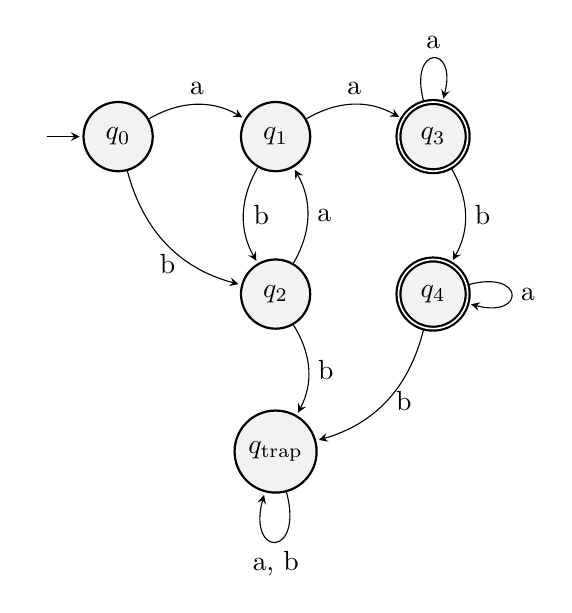
\begin{tikzpicture}[shorten >=1pt, node distance=2cm, on grid, auto]
        \node[state, initial] (q_0)   {$q_0$}; 
        \node[state] (q_1) [right=of q_0] {$q_1$}; 
        \node[state] (q_2) [below=of q_1] {$q_2$}; 
        \node[state, accepting] (q_3) [right=of q_1] {$q_3$}; 
        \node[state, accepting] (q_4) [right=of q_2] {$q_4$};
        \node[state] (trap) [below=of q_2] {$q_{\text{trap}}$};
    
        \path[->] 
        (q_0) edge [bend left, above] node {a} (q_1)
              edge [bend right, below] node {b} (q_2)
        (q_1) edge [bend left, above] node {a} (q_3)
              edge [bend right, right] node {b} (q_2)
        (q_2) edge [bend right, right] node {a} (q_1)
              edge [bend left, right] node {b} (trap)
         (q_3) edge [bend left, right] node {b} (q_4)
               edge [loop above] node {a} (q_3)
         (q_4) edge [loop right] node {a} (q_4)
               edge [bend left, right] node{b} (trap)

         
        (trap) edge [loop below] node {a, b} ();
    
    \end{tikzpicture}
   
   
  \end{solution}

  
\question[30] Given the languages, $A$ and $B$, we derive the language, $C = \{ w\in A \mid w \in B \}$.

  Prove or disprove the following claim.
  \begin{claim}
    If $A$ and $B$ are regular languages, then so is $C$.
  \end{claim}
  
  \begin{solution}
    We have to prove a language C has members : w is member of A given that it is member of B, where A and B are some regular languages then so is C. To accomplish this we can construct a DFA that accepts language C to complete the proof. 

    let $C' = (Q, \sigma, \delta, q_0, F)$ be a DFA that accepts language C. 
    Language A is accepted by DFA A' and language B is accepted by DFA B'
    Let $A' = (Q_A, \sigma, \delta_A, q_{0A}, F_A)$ and $B' = (Q_B, \sigma, \delta_B, q_{0B}, F_B)$

     We can construct C as follows:
    \begin{itemize}
      \item $Q = {(q_A, q_B) \mid q_A \in Q_A, q_B \in Q_B}$
      so the new state set Q is the cartesian product of the state sets of A and B.
      \item $\sigma = \sigma_A = \sigma_B$
      (since w $\in$ $\Sigma*$ and $\Sigma =\{a,b\}$ which is same for A and B)
      \item $\delta((q_A, q_B), a) = (\delta_A(q_A, a), \delta_B(q_B, a))$
      \item $q_0 = (q_{0A}, q_{0B})$
      \item $F = F_A \times F_B$
      the start states and end states of C' will be pair of start states and end states of A' and B' respectively.
    \end{itemize}
    Now we have to prove that C' is a DFA that accepts language C.
    \begin{itemize}
      \item C is a DFA because it has a finite set of states, a finite set of input symbols, a transition function, a start state, and a set of end states.
      \item C accepts language C because it accepts all strings w that are accepted by A and B.
    \end{itemize}
    Therefore, C is a DFA that accepts language C, so the claim is true.  

  \end{solution}
  
\question[35] Given the languages, $A$ and $B$, we define the following operation.
  \[
    A\smile_a B = \{ u\in A \mid \exists v\in B \ni n_a(u) = n_a(v) \}
  \]

  Prove or disprove the following claim.
  \begin{claim}
    The class of regular languages is closed under $\smile_a$.
  \end{claim}

  \begin{solution}
    To prove the claim, we need to show that the class of regular languages is closed under the $\smile_a$ operation. To do this, we need to show that for any two regular languages A and B, the language $A\smile_a B$ is also regular.
    For this proof, if we can construct a DFA that accepts the language $A\smile_a B$.
    Let $A' = (Q_A, \Sigma, \delta_A, q_{0A}, F_A)$ and $B' = (Q_B, \Sigma, \delta_B, q_{0B}, F_B)$ be the DFAs that accept languages A and B, respectively.
    However since the resulting language should should have equal number of a's from A and B in both strings so DFA cannot cater to dynamic nature and hence an NFA is required. Moreover, we have seen that an NFA can be converted to a DFA using subset construction. 
    Let $C'$ be an NFA that accepts C where C $=A \smile_a B$
    \begin{itemize}
      \item $Q =$ \{$(q1,q2) | q1 \in Q_A , q2 \in Q_B$ \} 
      or we can say that the new state set Q is the cartesian product of the state sets of A and B i.e. $Q = Q_A \times Q_B$
      \item $\Sigma_\epsilon = \Sigma_A \cup \epsilon = \Sigma_B \cup \epsilon $ \\
      For $q_a$ and $q_b$ $\in$ Q and t $\in$ $\Sigma_\epsilon$\\
        \[
       \delta((q_A, q_B), t) =
       \begin{cases} \{(\delta_A(q_a, t), \delta_B(q_B, t))\} when $  t = a$\\
       \{( \delta_A(q_a, b), q_b) \}  when $ t = b$\\
       \{( q_a, \delta_b(q_b, a), ) \}  when $ t = $\epsilon$ $\\
  
      \end{cases} \]
      \item $q_0 = (q_{0_A}, q_{0_B})$
      \item $F = F_A \times F_B$
      
      To enunciate the start state of C' is pair of start state of A' and B', \\
      End state F is also cartesian of end state of A' and B'\\
      $\delta(Q, t)$ is union of all possible states where on a given $\Sigma \in \Sigma_\epsilon $ transition function of A' and B' respectively can transition to. \\
  
    
    
      $L(C)$ is regular because it is accepted by an NFA and as per theorem 1.39 of our text book every NFA has a corresponding DFA, thus language C is regular. 
      Therefore, the claim is true.
      Hence, the class of regular languages is closed under the $\smile_a$ operation.
    \end{itemize}
    
  \end{solution}
\end{questions}

\end{document}

%%% Local Variables:
%%% mode: latex
%%% TeX-master: t
%%% End:
